\documentclass[12pt, a4paper]{article}
\usepackage[utf8]{inputenc}
\usepackage[]{graphicx}
\usepackage{indentfirst}
\pagenumbering{arabic}
\usepackage{fancyhdr}
\usepackage{amsmath}
\usepackage{amsfonts}
\usepackage{booktabs}
\usepackage{xcolor}
\usepackage{listings}
\usepackage{color}
\usepackage{caption}
\usepackage{lastpage}
\usepackage{tikz}
\usepackage{eso-pic}
\usetikzlibrary{calc}
\usetikzlibrary{decorations.pathmorphing}
\usepackage{array}
\definecolor{mygreen}{rgb}{0,0.6,0}
\definecolor{mygray}{rgb}{0.5,0.5,0.5}
\definecolor{mymauve}{rgb}{0.58,0,0.82}
\usepackage{longtable}
\usepackage{makecell}
\usepackage{float}
\usepackage{url}
\usepackage{hyperref}
\usepackage{adjustbox}
\usepackage{gensymb}
\usepackage{caption}
\usepackage{subcaption}
\usepackage{stackengine}
\usepackage[utf8]{inputenc}
\usepackage[vietnamese]{babel}

\hypersetup{
    colorlinks=true,
    linkcolor=blue,
    filecolor=magenta,      
    urlcolor=blue,
    pdfpagemode=FullScreen,
    }

\lstset{
  basicstyle=\ttfamily\footnotesize,
  breakatwhitespace=false,         
  breaklines=true,                 
  captionpos=b,                    
  keepspaces=true,                 
  numbers=left,                    
  numbersep=5pt,                  
  showspaces=false,                
  showstringspaces=false,
  showtabs=true,
  frame=shadowbox,
  tabsize=2
  commentstyle=\color{mygreen},
  keywordstyle=\color{blue},
  numberstyle=\tiny\color{mygray},
  rulecolor=\color{black},
  stringstyle=\color{mymauve},
}

\begin{document}

\begin{titlepage}

        \begin{tikzpicture}[overlay,remember picture]
        \draw [line width=3pt]
               ($ (current page.north west) + (1.5cm,-2.0cm) $)
            rectangle
            ($ (current page.south east) + (-1.5cm,2 .0 cm) $);
        \draw [line width=1pt]
            ($ (current page.north west) + (1.65cm,-2.15cm) $)
            rectangle
            ($ (current page.south east) + (-1.65cm,2.15cm) $); 
        \end{tikzpicture}%
        
	\centering
	
	{\scshape\large ĐẠI HỌC QUỐC GIA THÀNH PHỐ HỒ CHÍ MINH\\TRƯỜNG ĐẠI HỌC BÁCH KHOA \par}
	\vspace{0.5cm}
	\includegraphics[width=0.3\textwidth]{Images/Logo BK.png}\par\vspace{0.1 cm}
	{\scshape\large KHOA KHOA HỌC \& KỸ THUẬT MÁY TÍNH \\
	                Môn học: Hệ thống Thông minh\par} % Updated course name
	\vspace{1.5cm}

%%%%%% Your title goes here %%%%%%%%
	\begin{center}
	    \color{blue}
	    \begin{tabular}{c}
	    \hline
	    \\
	    \multicolumn{1}{l}{\large \bfseries Đề tài:}\\
	    \\
	    \Large \bfseries XÂY DỰNG ỨNG DỤNG \\ % Updated title
        \Large \bfseries CHẨN ĐOÁN SỚM VÀ THEO DÕI UNG THƯ PHỔI \\ % Updated title
	    \\
	    \hline
	    \end{tabular}
	\end{center}
%%%%%%%%%%%%%%%%%%%%%%%%%%%%%%%%%%%
%-------Your name goes here --------
%-------Your MSSV goes here --------

	\vspace{1cm}
	\begin{center}
	    \large 
	    \begin{tabular}{l l l}
	        Giảng viên hướng dẫn:   &  TS. Trần Tuấn Anh &\\
	        Học viên:   &  Đặng Linh Anh & 2370113\\
	    \end{tabular}
	    
	\end{center}
    \vspace{1.5cm}
%%%%%%%%%%%%%%%%%%%%%%%%%%%%%%%%%%%    
	\vfill
	{ TP. Hồ Chí Minh, ngày 28 tháng 4 năm 2025 } % Updated date
\end{titlepage}
\newpage
%%%%%%%%%%%%%%%%%%%%%%%%%%%%%%%%%%%
%-------------- Headnote and footnote ------- 
\pagestyle{fancy}
\fancyhead{} % clear all header fields
\fancyhead[L]{
 \begin{tabular}{rl}
    \begin{picture}(15,15)(0, 4)
    \put(0,-8){\includegraphics[width=10mm, height=10mm]{Images/Logo BK.png}}
    %\put(0,-8){\epsfig{width=10mm,figure=hcmut.eps}}
   \end{picture}&
	%\includegraphics[width=8mm, height=8mm]{hcmut.png} & %
	\begin{tabular}{l}
		\textbf{\bf \ttfamily Trường đại học Bách Khoa }\\
		\textbf{\bf \ttfamily Khoa Khoa học \& Kỹ thuật Máy tính}
	\end{tabular} 	
 \end{tabular}
}
\fancyhead[R]{
	\begin{tabular}{l}
		\tiny \bf \\
		\tiny \bf 
	\end{tabular}  }
\fancyfoot{} % clear all footer fields
\fancyfoot[L]{\scriptsize  \ttfamily 
% \begin{tabular}{l}
%      Exercise for Mathematical Foundation for Computer Science  \\
% \end{tabular}
}
%-----------Remember to modify the page when finished ------
\fancyfoot[R]{\scriptsize \ttfamily  Page {\thepage}/\pageref{LastPage}}
%-----------Remember to modify the page when finished ------

\renewcommand{\headrulewidth}{0.3pt}
\renewcommand{\footrulewidth}{0.3pt}
\AddToHook{cmd/section/before}{\clearpage}
\tableofcontents
\newpage

% Input sections based on report.md outline
\section{Introduction}
LungWise, the Lung Cancer Early Diagnosis and Monitoring application, is a web-based tool designed to help doctors detect early signs of lung cancer by combining AI-driven risk predictions with traditional clinical assessments. By gathering patient data, summarizing symptoms, and tracking diagnostic history, the application improves decision-making quality and streamlines future monitoring.

Code and dataset: \href{https://github.com/anhdang000/lungwise-IntelligentSystem}{GITHUB}

Youtube presentation video: \href{https://youtu.be/m5jL2PAiXLk}{YOUTUBE}

\section{Các bên liên quan và lợi ích}
\begin{itemize}
    \item \textbf{Bác sĩ và nhân viên y tế:}
    \begin{itemize}
        \item \textit{Hỗ trợ quyết định lâm sàng:} Nhận diện nhanh chóng các bệnh nhân có nguy cơ ung thư phổi cao dựa trên phân tích AI, giúp tập trung nguồn lực và sự chú ý.
        \item \textit{Nâng cao độ chính xác chẩn đoán:} Tích hợp dự đoán AI với đánh giá lâm sàng để đưa ra chẩn đoán chính xác hơn, giảm thiểu sai sót.
        \item \textit{Tối ưu hóa quy trình làm việc:} Giảm thời gian cần thiết để xem xét hồ sơ bệnh án phức tạp nhờ giao diện tổng hợp thông tin trực quan.
        \item \textit{Cải thiện giao tiếp với bệnh nhân:} Có thêm công cụ để giải thích rõ ràng về nguy cơ và kế hoạch theo dõi cho bệnh nhân.
    \end{itemize}
    
    \item \textbf{Bệnh nhân:}
    \begin{itemize}
        \item \textit{Phát hiện sớm bệnh:} Tăng cơ hội phát hiện ung thư phổi ở giai đoạn đầu, cải thiện đáng kể tiên lượng và khả năng điều trị thành công.
        \item \textit{Kế hoạch theo dõi cá nhân hóa:} Nhận được lịch trình và phương pháp theo dõi phù hợp với mức độ nguy cơ và tình trạng sức khỏe cụ thể.
        \item \textit{Can thiệp kịp thời:} Giảm nguy cơ bệnh tiến triển nặng nhờ việc theo dõi sát sao và can thiệp y tế đúng lúc.
        \item \textit{Tăng cường sự an tâm:} Hiểu rõ hơn về tình trạng sức khỏe của mình và cảm thấy yên tâm hơn với quy trình chăm sóc chủ động.
    \end{itemize}

    \item \textbf{Quản trị viên bệnh viện và phòng khám:}
    \begin{itemize}
        \item \textit{Giám sát hiệu quả hoạt động:} Truy cập các báo cáo và bảng điều khiển tổng hợp để theo dõi hiệu quả của chương trình sàng lọc và chẩn đoán.
        \item \textit{Phân bổ nguồn lực tối ưu:} Đưa ra quyết định dựa trên dữ liệu về việc phân bổ nhân lực, thiết bị và ngân sách cho hoạt động chăm sóc bệnh nhân ung thư phổi.
        \item \textit{Đảm bảo và nâng cao chất lượng dịch vụ:} Sử dụng dữ liệu hiệu suất để chứng minh sự tuân thủ các tiêu chuẩn chất lượng y tế và xác định các lĩnh vực cần cải thiện.
        \item \textit{Hỗ trợ lập kế hoạch chiến lược:} Cung cấp thông tin chi tiết về xu hướng bệnh tật và hiệu quả can thiệp, hỗ trợ xây dựng chiến lược y tế dài hạn.
    \end{itemize}

    \item \textbf{Nhà khoa học dữ liệu và nhà phát triển:}
    \begin{itemize}
        \item \textit{Tinh chỉnh và cải tiến mô hình AI:} Kiến trúc mô-đun và quy trình dữ liệu rõ ràng cho phép dễ dàng thử nghiệm, đánh giá và cập nhật các mô hình dự đoán.
        \item \textit{Phát triển và mở rộng tính năng:} Nhanh chóng tích hợp các nguồn dữ liệu mới (ví dụ: hình ảnh y tế) hoặc thêm các chức năng hỗ trợ quyết định khác.
        \item \textit{Triển khai liền mạch các dịch vụ AI mới:} Dễ dàng tích hợp các thuật toán hoặc công nghệ AI tiên tiến khác vào hệ thống hiện có.
        \item \textit{Bảo trì và nâng cấp hệ thống hiệu quả:} Thiết kế hệ thống rõ ràng giúp đơn giản hóa việc sửa lỗi, bảo trì và nâng cấp phần mềm.
    \end{itemize}

    \item \textbf{Cơ quan quản lý và công ty bảo hiểm:}
    \begin{itemize}
        \item \textit{Đảm bảo tuân thủ quy định:} Cung cấp dấu vết kiểm toán minh bạch và tài liệu hóa quy trình để chứng minh sự tuân thủ các quy định về quyền riêng tư dữ liệu (ví dụ: HIPAA, GDPR) và an toàn y tế.
        \item \textit{Xác thực độ tin cậy của mô hình:} Truy cập các chỉ số hiệu suất tổng hợp để đánh giá tính công bằng, độ chính xác và độ tin cậy của các thuật toán AI được sử dụng.
        \item \textit{Đánh giá hiệu quả chi phí:} Phân tích dữ liệu để xác định lợi tức đầu tư và hiệu quả chi phí của việc triển khai hệ thống chẩn đoán sớm dựa trên AI.
        \item \textit{Quản lý rủi ro và chính sách:} Thông tin từ hệ thống có thể hỗ trợ việc xây dựng các chính sách y tế và bảo hiểm dựa trên bằng chứng.
    \end{itemize}
\end{itemize}

\section{Algorithm Theory}

In machine learning, classification is a common task that aims to assign a category label to an input data sample based on its features. There are many different classification algorithms, each with its own strengths and weaknesses, suitable for different types of data and problems.

\subsection{Common Classification Algorithms}
Some commonly used classification algorithms include:
\begin{itemize}
    \item \textbf{Logistic Regression:} A simple but effective linear model, often used as a baseline. It models the probability of a binary class using the sigmoid function.
    \item \textbf{Support Vector Machine (SVM):} Searches for an optimal hyperplane to separate data classes in feature space. SVM is effective in high-dimensional spaces and when the number of dimensions is greater than the number of samples.
    \item \textbf{Decision Tree:} Builds a tree-like model where each internal node represents a test on a feature, each branch represents the outcome of the test, and each leaf node represents a class label. Decision trees are easy to interpret but prone to overfitting.
    \item \textbf{Random Forest:} An ensemble learning algorithm that builds multiple decision trees during training and outputs the mode of the classes (for classification) or mean prediction (for regression) of the individual trees. It reduces the overfitting problem of single decision trees.
    \item \textbf{Naïve Bayes:} Based on Bayes' theorem with a "naïve" assumption of conditional independence between features. It is simple, fast, and works well on large datasets.
    \item \textbf{Gradient Boosting Machines (GBM):} Another ensemble learning technique that builds models (usually decision trees) sequentially, with each new model trying to correct the errors of previous models. Popular variations include AdaBoost, Gradient Boosting, and XGBoost.
\end{itemize}

\subsection{Choosing XGBoost}

In this project, we chose XGBoost (eXtreme Gradient Boosting) as the main classification algorithm for the following reasons:
\begin{itemize}
    \item \textbf{High Performance:} XGBoost consistently achieves top results in machine learning competitions and is known for high prediction accuracy on tabular data.
    \item \textbf{Optimization and Speed:} The XGBoost library is highly optimized for speed and memory usage. It implements techniques such as parallel computing, handling of missing values, and efficient tree pruning.
    \item \textbf{Overfitting Prevention:} XGBoost incorporates regularization techniques such as L1 (Lasso) and L2 (Ridge) directly into its objective function, helping to minimize overfitting and improve model generalization.
    \item \textbf{Handling Missing Values:} XGBoost has built-in mechanisms to handle missing values in data, simplifying the preprocessing process.
    \item \textbf{Flexibility:} XGBoost supports custom objective and evaluation functions, allowing model fine-tuning for specific problems.
\end{itemize}

Compared to other algorithms, XGBoost provides a good balance between accuracy, speed, and overfitting control, making it especially suitable for the tabular medical data used in this project.

\subsection{Overview of XGBoost}
XGBoost is an optimized implementation of the Gradient Boosting algorithm. Key concepts include:
\begin{itemize}
    \item \textbf{Gradient Boosting:} An ensemble machine learning method that builds prediction models as a combination of weak prediction models (usually decision trees). It builds trees sequentially, with each new tree learning to correct the errors (residuals) of the previous tree set. Unlike AdaBoost which adjusts data point weights, Gradient Boosting adjusts the model based on the gradient of the loss function.
    \item \textbf{Regularization:} To prevent overfitting, XGBoost adds regularization components to its objective function. This includes both L1 regularization (helping reduce the number of features) and L2 regularization (helping reduce the magnitude of leaf weights), making the model generalize better on unseen data.
    \item \textbf{Tree Pruning and Sparsity Awareness:} XGBoost uses an efficient approximation algorithm to find optimal split points and performs tree pruning based on the maximum negative gain. It is also designed to handle missing values in data efficiently by learning default directions at each node.
    \item \textbf{System Optimization:} XGBoost leverages hardware and software optimization techniques such as parallel computing (using all CPU cores), distributed computing, memory cache optimization, and out-of-core computation to process large datasets efficiently.
\end{itemize}
The combination of these techniques helps XGBoost deliver high prediction performance and good scalability for structured tabular data, making it a suitable choice for the early diagnosis of lung cancer.

\section{System Design}

The Lung Cancer Early Diagnosis and Monitoring system is designed using a modern client-server architecture, consisting of three main components: User Interface (Frontend), Backend Services, and Database.

\subsection{User Interface (UI) Design}

The user interface is built to provide an intuitive and efficient experience for doctors and medical staff.
\begin{itemize}
    \item \textbf{Core Technologies:} React \cite{react} and TypeScript \cite{typescript}. React was chosen for its rich ecosystem and ability to create dynamic user interfaces. TypeScript enhances code reliability and maintainability through static type checking.
    \item \textbf{Styling:} Tailwind CSS \cite{tailwindcss} is used for quick and consistent styling. It allows building highly customized interfaces without writing much custom CSS.
    \item \textbf{Component Library:} Using a UI component library (e.g., Shadcn/ui \cite{shadcnui} or similar) to provide pre-built components like cards, forms, charts, and tables, helping to speed up development and ensure interface consistency.
    \item \textbf{UI Theme:} Applying a color scheme with light blue tones as the main colors. These colors were chosen to create a sense of trust, professionalism, and readability in clinical settings, reducing eye strain during long periods of use.
\end{itemize}

\subsection{User Flows}
This section describes the main interaction flows of users (doctors) with the system.
\begin{itemize}
    \item \textbf{Overview Flow:} Doctors log in and view the main dashboard with a list of patients and alerts.
    \item \textbf{Patient Detail Flow:} Doctors select a patient from the list to view detailed information, symptom history, and the latest AI prediction results.
    \item \textbf{Information Update Flow:} Doctors update new symptoms or monitoring notes for patients.
\end{itemize}
% (Optional: Add user flow diagram images here if available)
% \begin{figure}[h]
%     \centering
%     \includegraphics[width=0.8\textwidth]{Images/user_flow_diagram.png}
%     \caption{Flow diagram for viewing patient details.}
%     \label{fig:user_flow}
% \end{figure}

\subsection{Mockups}
The images below illustrate the user interface design for the main screens of the application.

\begin{figure}[h]
    \centering
    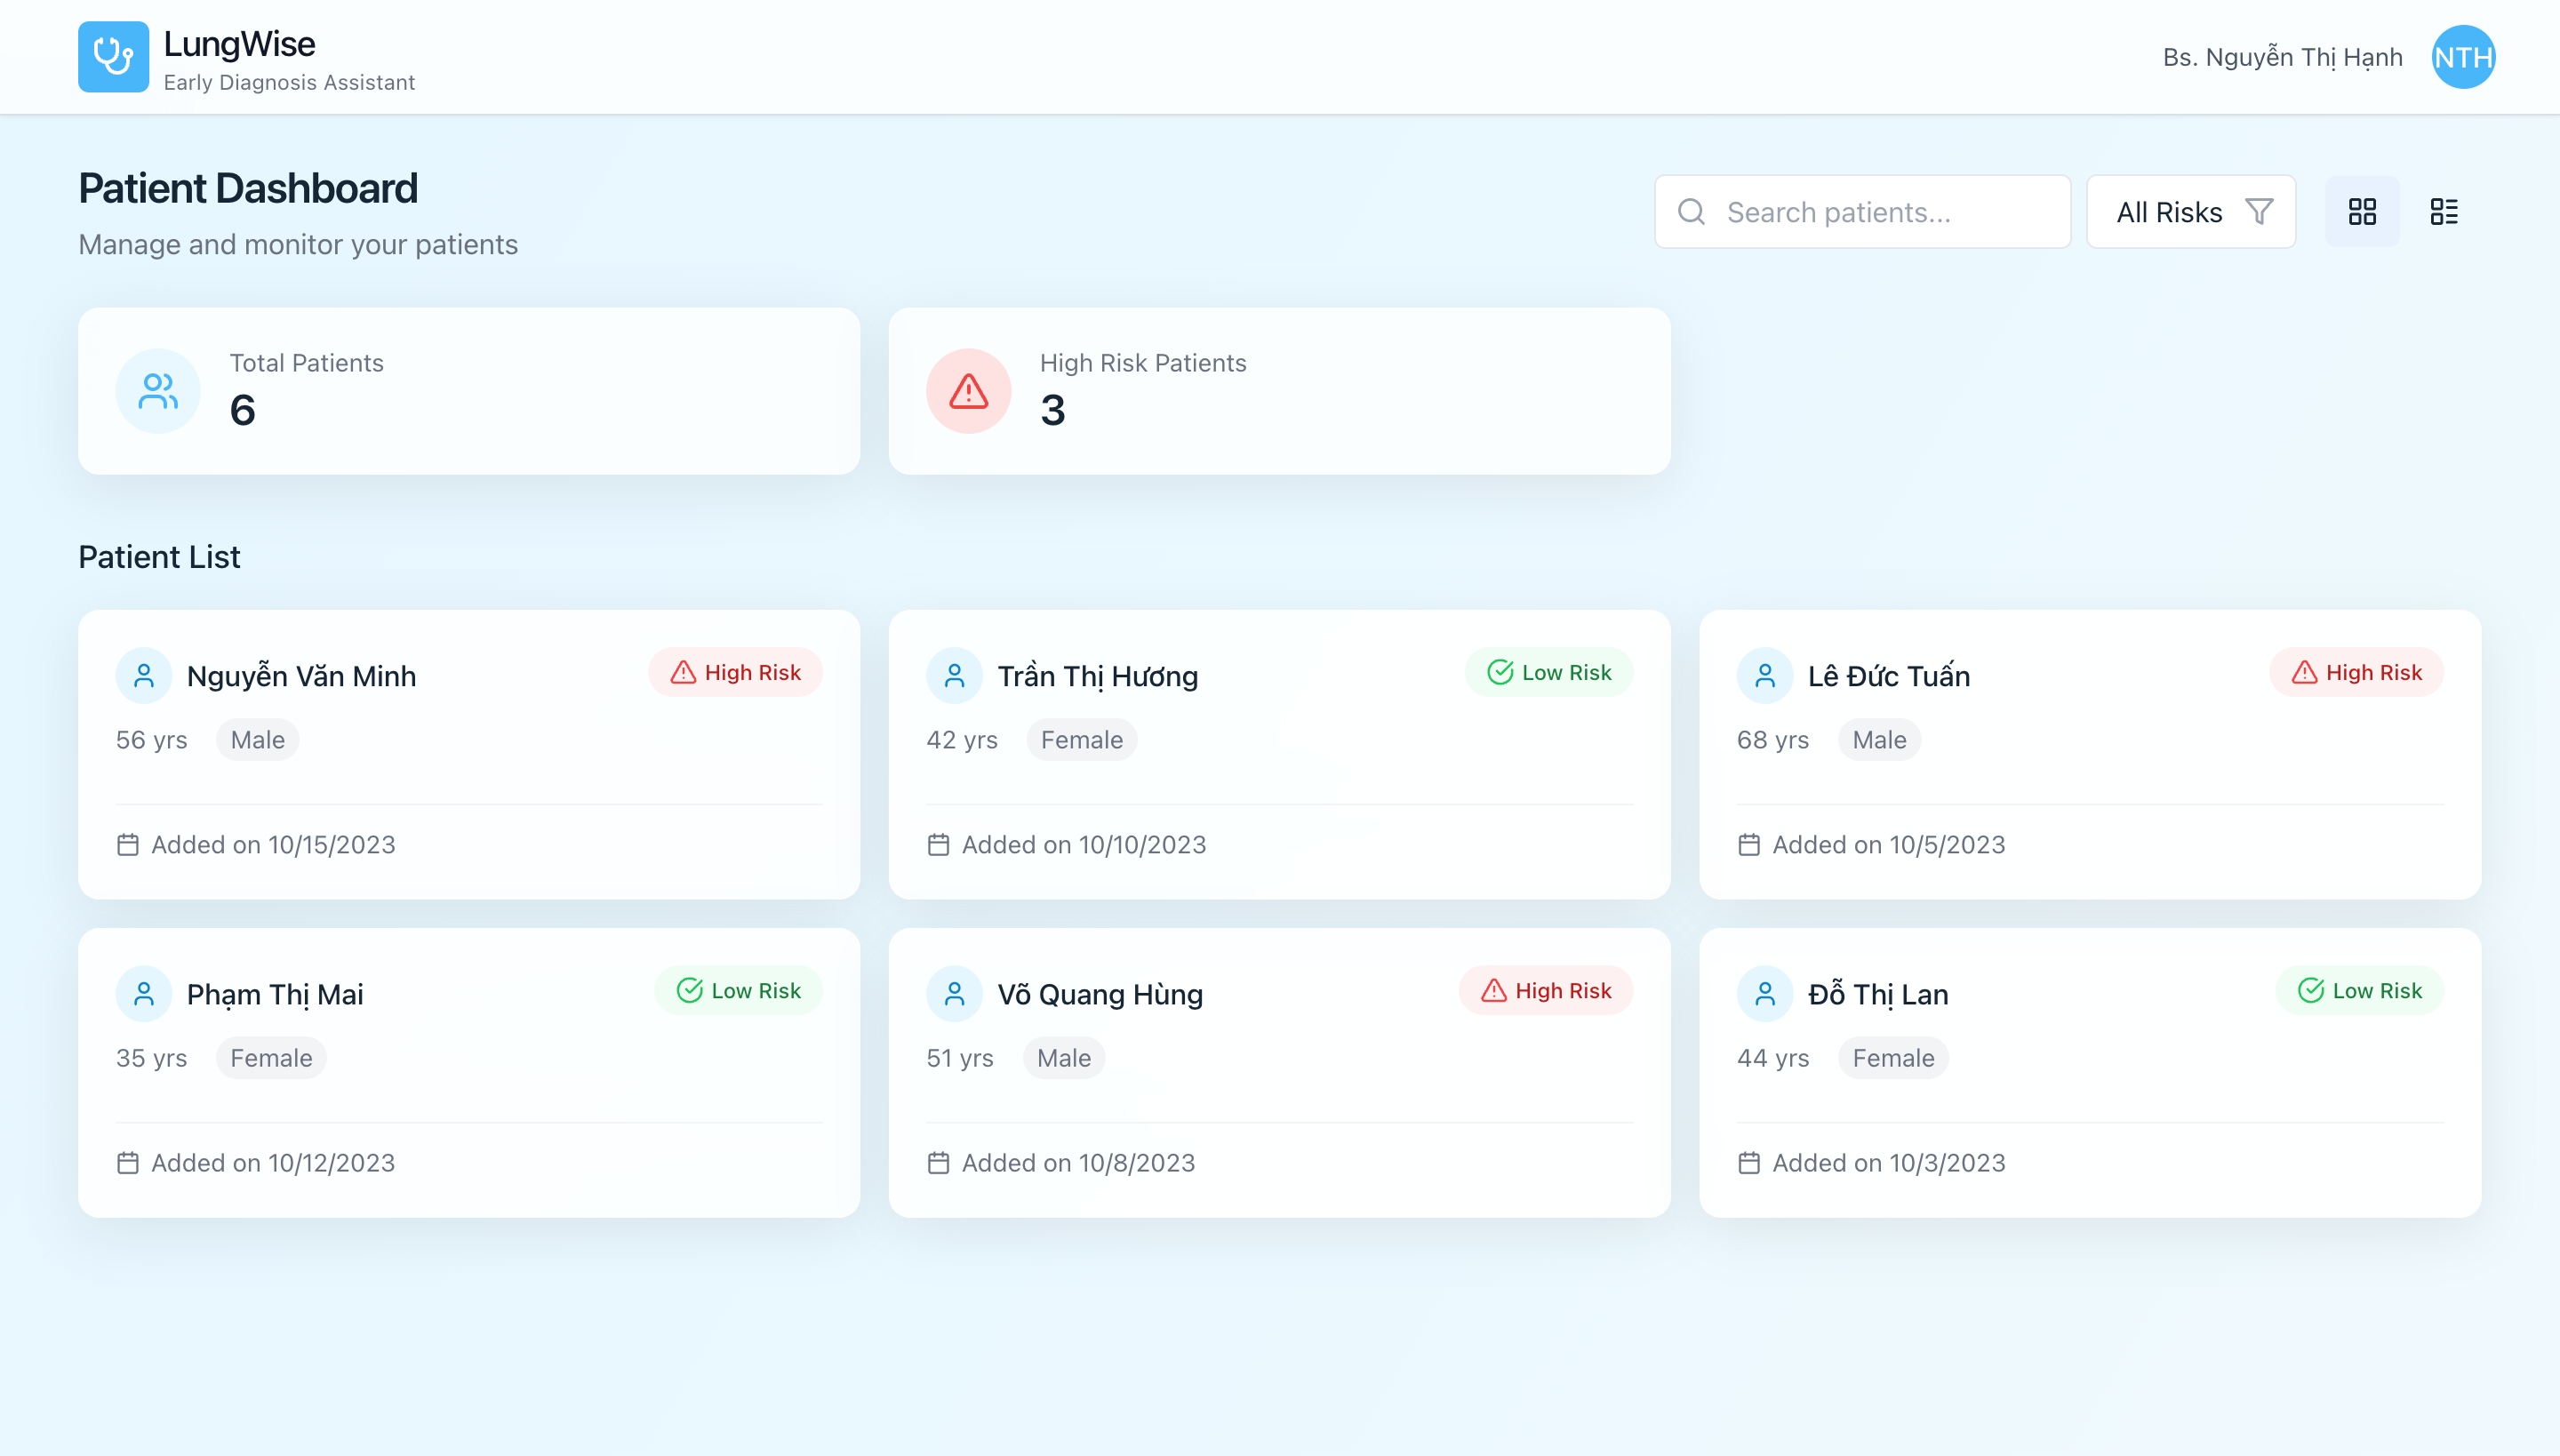
\includegraphics[width=0.9\textwidth]{Images/dashboard.png}
    \caption{The main patient dashboard interface showing patient list, risk categorization, and filtering options.}
    \label{fig:dashboard_mockup}
\end{figure}

\begin{figure}[h]
    \centering
    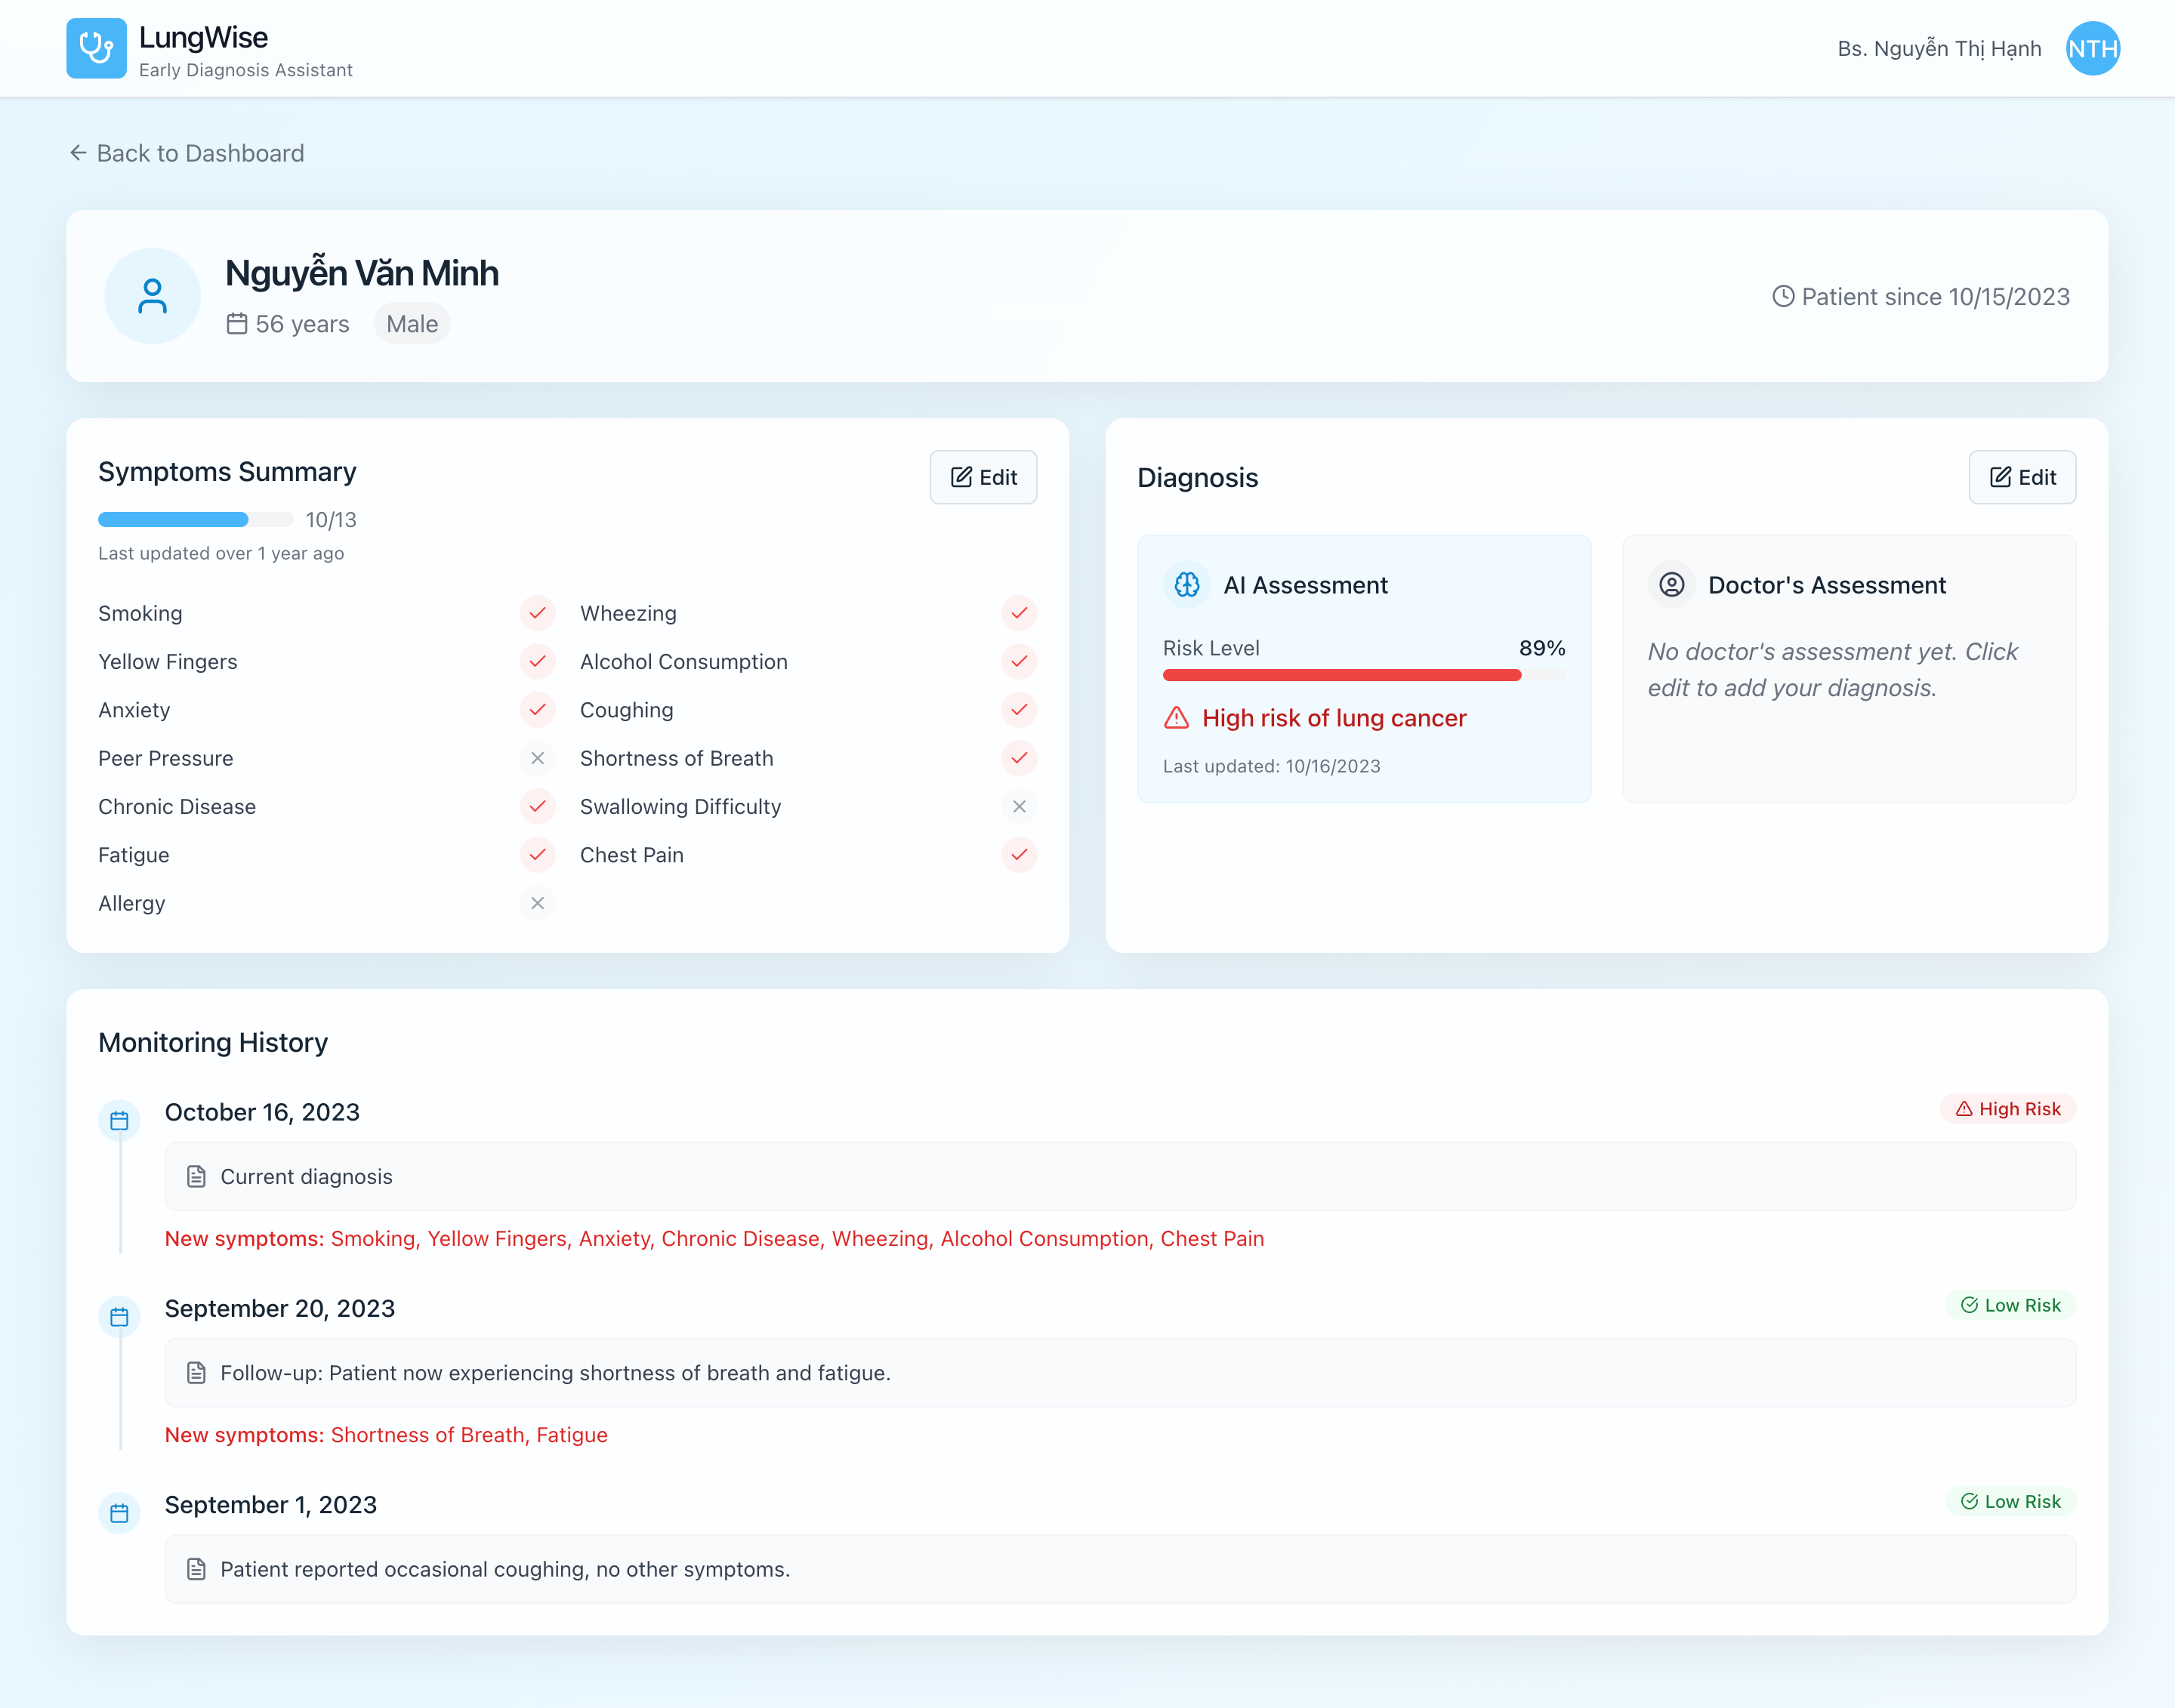
\includegraphics[width=0.9\textwidth]{Images/patient_detail.png}
    \caption{Patient detail interface showing personal information, symptoms summary, diagnostic assessment, and monitoring history.}
    \label{fig:patient_detail_mockup}
\end{figure}

\begin{figure}[h]
    \centering
    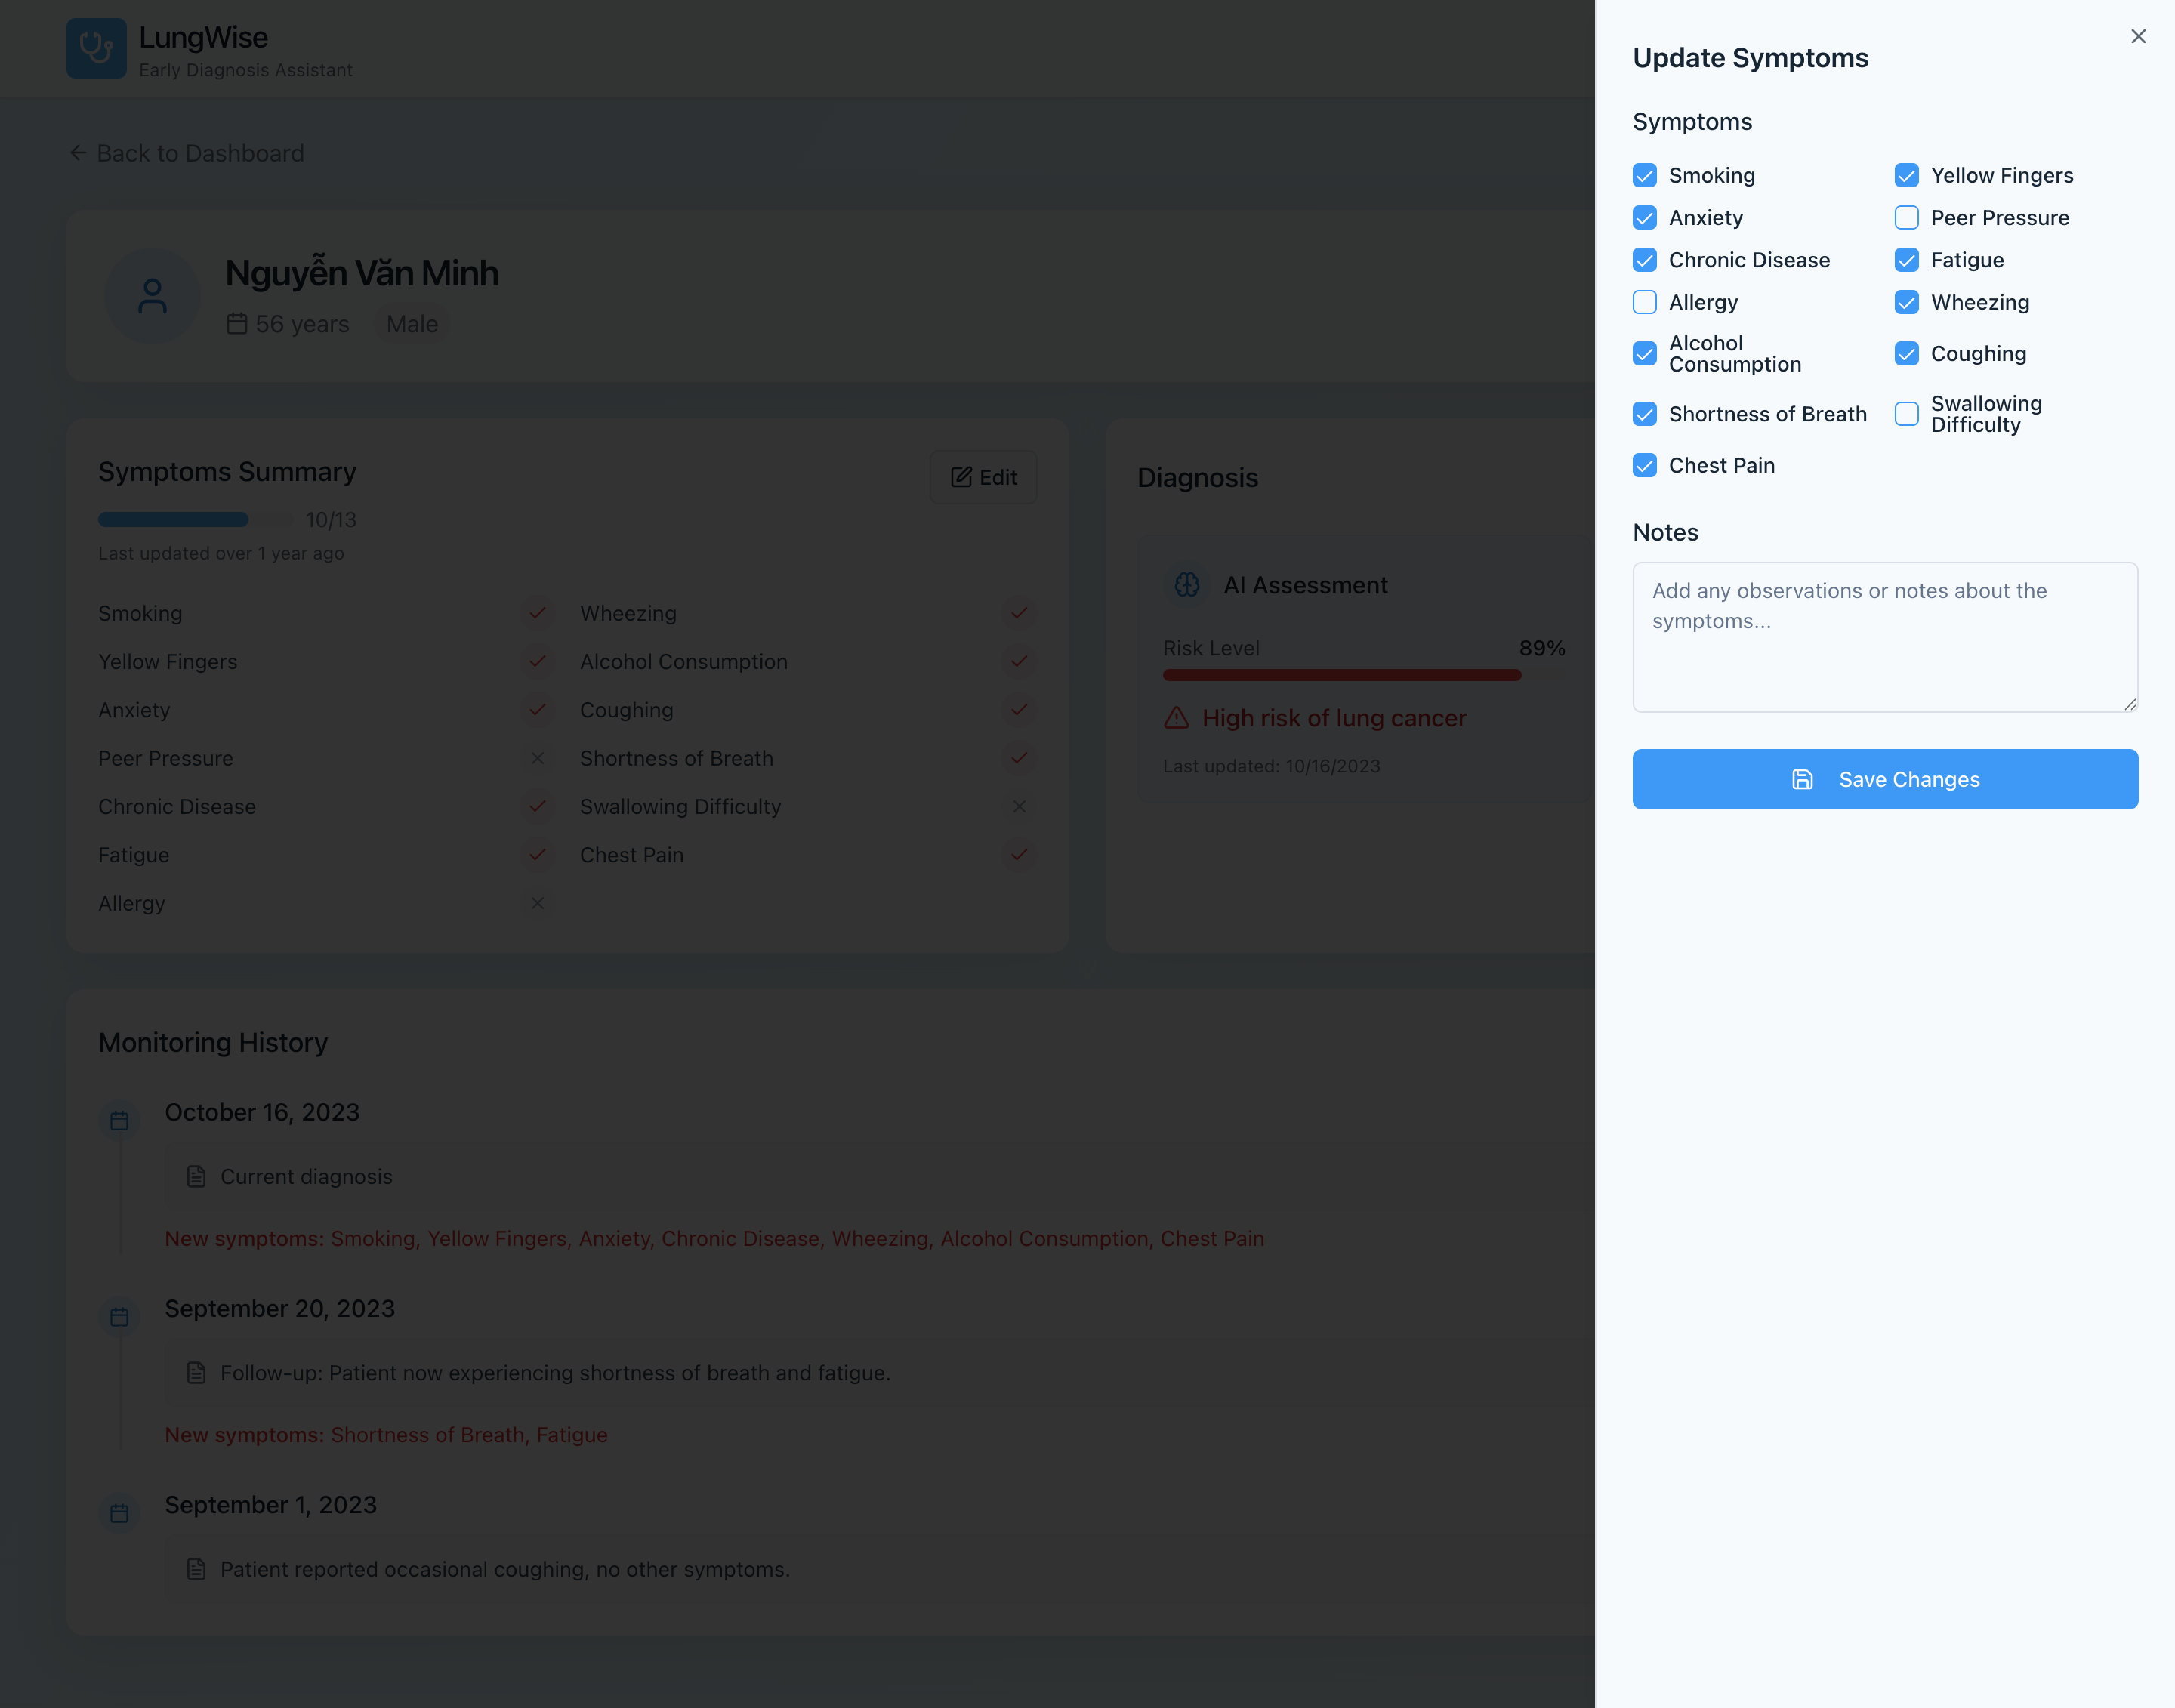
\includegraphics[width=0.9\textwidth]{Images/patient_update_symptoms.png}
    \caption{Patient symptom update interface allowing healthcare providers to record current symptoms and their severity.}
    \label{fig:symptom_update}
\end{figure}

\begin{figure}[h]
    \centering
    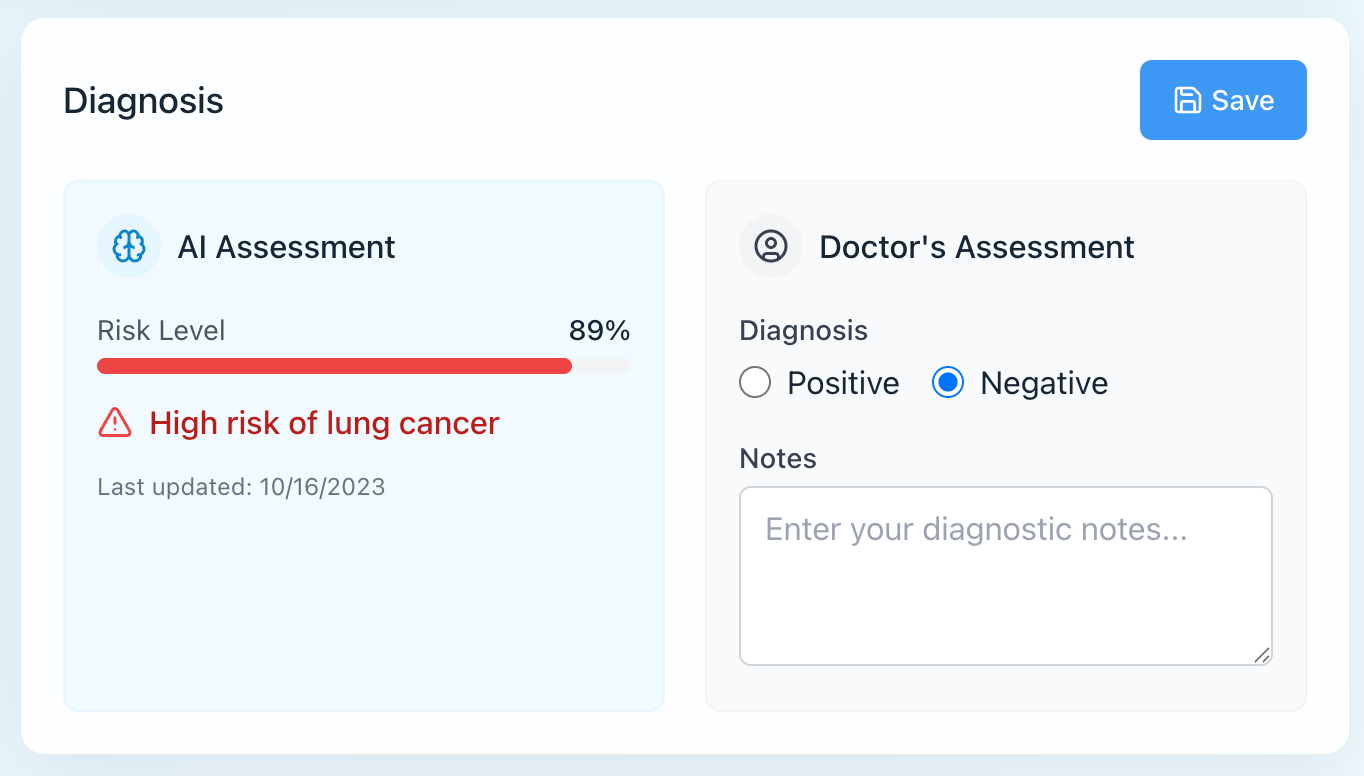
\includegraphics[width=0.9\textwidth]{Images/doctor_feedback_box.png}
    \caption{Doctor feedback interface where physicians can provide their clinical assessment and treatment recommendations based on updated symptoms and AI risk prediction.}
    \label{fig:doctor_feedback}
\end{figure}

\subsection{Backend Services}

The backend service plays a central role, handling business logic, data management, and interaction with the AI model. It provides a RESTful application programming interface (API) for the frontend to interact with.
\begin{itemize}
    \item \textbf{Core Technology:} FastAPI \cite{fastapi} (Python). FastAPI was chosen for its high performance, modern syntax based on Python type hints, and ability to automatically generate API documentation (Swagger UI/ReDoc).
    \item \textbf{Deployment:} The backend system is packaged as Docker \cite{docker} services, facilitating deployment, management, and scaling across different environments.
    \item \textbf{Key APIs:} The main RESTful endpoints include:
        \begin{itemize}
            \item \texttt{GET /patients}: Get a list of patients (supports search and filtering).
            \item \texttt{GET /patients/\{patient\_id\}}: Get detailed information about a specific patient.
            \item \texttt{POST /patients}: Create a new patient record.
            \item \texttt{PUT /patients/\{patient\_id\}}: Update patient information.
            \item \texttt{GET /patients/\{patient\_id\}/history}: Get monitoring history (diagnoses, old symptoms) of a patient.
            \item \texttt{POST /patients/\{patient\_id\}/diagnoses}: Add a new diagnosis record, including calling the AI model to get risk prediction and storing the results along with doctor's notes.
            \item \texttt{POST /patients/\{patient\_id\}/symptoms}: Update current patient symptoms.
            \item \texttt{POST /predict}: Receive patient data (features) and return lung cancer risk prediction from the XGBoost \cite{chen2016xgboost} model. (Usually called internally when creating a new diagnosis, but can be provided separately if needed).
            \item \texttt{GET /model/info}: Get information about the ML model version being used (e.g., training date, key performance metrics).
            \item \texttt{POST /explain}: Receive patient data and return explanation for the prediction (e.g., using SHAP values to identify most influential features).
            \item \texttt{POST /retrain}: Trigger the ML model retraining process (typically protected and only for administrators or automated processes).
            \item \textit{(User authentication is handled through integrated Supabase \cite{supabase} Auth.)}
        \end{itemize}
\end{itemize}

\subsection{Database}

The database stores all important information for the system.
\begin{itemize}
    \item \textbf{Database Management System:} PostgreSQL \cite{postgresql} was chosen as the main relational database. PostgreSQL is known for its reliability, rich features, and scalability, making it suitable for storing structured data such as patient records, symptom logs, and monitoring events.
    \item \textbf{Real-time Updates:} Leveraging Supabase's \cite{supabase} real-time subscriptions feature (or a similar PostgreSQL-based solution) to push data updates (e.g., new prediction results, changed patient information) from backend to client automatically, ensuring the user interface always displays the latest information without manual refreshing.
\end{itemize}

\subsection{System Architecture Diagram}

Figure \ref{fig:system_architecture} illustrates the overall architecture and interaction between the different components of the LungWise application.

\begin{figure}[h]
    \centering
    \begin{tikzpicture}[
        node distance=1.5cm and 3cm,
        box/.style={draw, rounded corners, minimum width=3cm, minimum height=1.5cm, fill=blue!10, text width=3cm, align=center},
        arrow/.style={->, >=latex, thick},
        database/.style={cylinder, draw, shape border rotate=90, aspect=0.3, minimum width=1.5cm, minimum height=2cm, fill=green!10, text width=1.5cm, align=center},
        model/.style={ellipse, draw, minimum width=2cm, minimum height=1.5cm, fill=orange!20, text width=2.5cm, align=center}
    ]
    
    % Client tier
    \node[box, fill=blue!10] (ui) {User Interface\\(React, TypeScript)};
    \node[below=0.2cm of ui, align=center] (uitech) {\small Tailwind CSS\\Shadcn/UI};
    
    % Server tier
    \node[box, fill=purple!10, right=of ui] (api) {Backend API\\(FastAPI, Python)};
    \node[below=0.2cm of api, align=center] (apitech) {\small REST Endpoints\\JWT Auth};
    
    % Model tier
    \node[model, below right=of api] (model) {ML Model\\(XGBoost)};
    
    % Data tier
    \node[database, below left=of api] (db) {Database\\(PostgreSQL)};
    
    % Connections
    \draw[arrow] (ui) -- node[above] {\small HTTP/REST} (api);
    \draw[arrow] (api) -- node[left] {\small CRUD} (db);
    \draw[arrow] (db) -- node[below] {\small Patient Data} ([xshift=-1cm]api.south);
    \draw[arrow] (api) -- node[right] {\small Features} (model);
    \draw[arrow] (model) -- node[below] {\small Predictions} ([xshift=1cm]api.south);
    \draw[arrow] ([xshift=1.5cm]api.west) -- node[below] {\small JSON} ([xshift=-1.5cm]ui.east);
    
    % Real-time subscription
    \draw[arrow, dashed] (db) to[out=180, in=240] node[left] {\small Real-time\\Updates} (ui);
    
    % User
    \node[left=of ui, align=center] (user) {\includegraphics[width=1cm]{Images/doctor-icon.png}\\Doctor};
    \draw[arrow] (user) -- (ui);
    
    % System boundary
    \node[draw, dashed, fit=(ui) (uitech) (api) (apitech) (db) (model), inner sep=0.5cm, rounded corners] (system) {};
    \node[above] at (system.north) {LungWise System};
    
    \end{tikzpicture}
    \caption{System architecture diagram of the LungWise application showing the interaction between the user interface, backend services, machine learning model, and database.}
    \label{fig:system_architecture}
\end{figure}

As shown in the diagram, the LungWise system follows a modern three-tier architecture with clear separation of concerns:

\begin{itemize}
    \item The \textbf{Client Tier} consists of the React \cite{react}/TypeScript \cite{typescript} frontend that doctors interact with. It communicates with the backend via HTTP/REST calls and receives real-time updates through a subscription mechanism.
    
    \item The \textbf{Server Tier} contains the FastAPI \cite{fastapi} backend that processes requests, enforces business logic, and orchestrates data flow between the client, database, and ML model.
    
    \item The \textbf{Data Tier} includes both the PostgreSQL \cite{postgresql} database for persistent storage and the XGBoost \cite{chen2016xgboost} model for risk predictions. The model leverages scikit-learn \cite{pedregosa2011scikit} for preprocessing and evaluation pipelines.
\end{itemize}

This architecture provides several advantages:
\begin{itemize}
    \item \textbf{Scalability:} Each component can be scaled independently based on demand.
    \item \textbf{Maintainability:} Changes to one tier (e.g., updating the ML model) can be made without affecting other tiers.
    \item \textbf{Security:} Sensitive operations and data access are handled on the server, not exposed to the client.
    \item \textbf{Real-time capabilities:} Users receive immediate updates when data changes.
\end{itemize}

\section{Tập dữ liệu và tiền xử lý}

Chất lượng của mô hình dự đoán phụ thuộc rất nhiều vào chất lượng và cách xử lý dữ liệu đầu vào. Phần này mô tả nguồn dữ liệu, các đặc trưng được thu thập và các bước tiền xử lý được thực hiện.

\subsection{Nguồn dữ liệu}

Dữ liệu được sử dụng trong dự án này là tập hợp các hồ sơ bệnh nhân lịch sử, bao gồm thông tin về nhân khẩu học, yếu tố lối sống và các triệu chứng lâm sàng liên quan đến ung thư phổi. Nguồn dữ liệu này (ví dụ: từ một nghiên cứu hoặc cơ sở dữ liệu bệnh viện cụ thể) cần được nêu rõ nếu có thể.

\subsection{Các đặc trưng được thu thập}

Các đặc trưng sau đây đã được thu thập cho mỗi bệnh nhân:
\begin{itemize}
    \item \textbf{Nhân khẩu học:} Giới tính (GENDER), Tuổi (AGE).
    \item \textbf{Lối sống:} Hút thuốc (SMOKING), Sử dụng rượu (ALCOHOL CONSUMING).
    \item \textbf{Yếu tố nguy cơ và triệu chứng:} Vàng ngón tay (YELLOW\_FINGERS), Lo lắng (ANXIETY), Áp lực từ bạn bè/đồng nghiệp (PEER\_PRESSURE), Bệnh mãn tính (CHRONIC DISEASE), Mệt mỏi (FATIGUE), Dị ứng (ALLERGY), Thở khò khè (WHEEZING), Ho (COUGHING), Khó thở (SHORTNESS OF BREATH), Khó nuốt (SWALLOWING DIFFICULTY), Đau ngực (CHEST PAIN).
    \item \textbf{Nhãn mục tiêu:} Chẩn đoán ung thư phổi (LUNG\_CANCER) - xác nhận bệnh nhân có bị ung thư phổi hay không.
\end{itemize}

\subsection{Các bước làm sạch và tiền xử lý dữ liệu}

Để chuẩn bị dữ liệu cho việc huấn luyện mô hình, các bước sau đã được thực hiện:
\begin{itemize}
    \item \textbf{Xử lý giá trị thiếu:} Các bản ghi có giá trị bị thiếu đã được xử lý bằng cách loại bỏ hoặc sử dụng các kỹ thuật điền khuyết (imputation) phù hợp (ví dụ: điền bằng giá trị trung bình, trung vị hoặc mode).
    \item \textbf{Mã hóa biến hạng mục (Categorical Encoding):} Các đặc trưng hạng mục (ví dụ: Giới tính) đã được chuyển đổi thành dạng số bằng kỹ thuật mã hóa one-hot (one-hot encoding).
    \item \textbf{Chuẩn hóa biến liên tục (Continuous Variable Standardization):} Các đặc trưng liên tục (ví dụ: Tuổi) đã được chuẩn hóa (ví dụ: sử dụng Z-score standardization) để có giá trị trung bình bằng 0 và độ lệch chuẩn bằng 1, giúp các thuật toán học máy hoạt động hiệu quả hơn.
\end{itemize}

\subsection{Kỹ thuật đặc trưng (Feature Engineering)}

Một số kỹ thuật đặc trưng đơn giản đã được áp dụng:
\begin{itemize}
    \item \textbf{Tạo cờ nhị phân (Binary Flags):} Chuyển đổi các đặc trưng triệu chứng thành dạng cờ nhị phân (0 hoặc 1) để biểu thị sự có mặt hay vắng mặt của triệu chứng.
    \item \textbf{Tổng hợp điểm rủi ro (Composite Score - tùy chọn):} Có thể xem xét việc tạo ra một điểm số rủi ro tổng hợp dựa trên sự kết hợp của các yếu tố nguy cơ đã biết (ví dụ: tuổi, hút thuốc, bệnh mãn tính). Tuy nhiên, trong nhiều trường hợp, để mô hình tự học các mối quan hệ phức tạp sẽ hiệu quả hơn.
\end{itemize}

\subsection{Phân chia tập dữ liệu Huấn luyện - Kiểm tra (Train-Test Split)}

Tập dữ liệu đã được chia thành hai phần: tập huấn luyện (80%) và tập kiểm tra (20%). Việc phân chia được thực hiện bằng phương pháp phân chia có phân tầng (stratified split) để đảm bảo rằng tỷ lệ các trường hợp ung thư phổi (lớp dương tính) trong cả hai tập dữ liệu là tương đương nhau. Điều này rất quan trọng đối với các tập dữ liệu mất cân bằng để đánh giá mô hình một cách chính xác.

\section{Evaluation Results}

The performance of the XGBoost model was evaluated on the hold-out test set using standard evaluation metrics for classification problems.

\subsection{Key Performance Metrics}

The main performance metrics of the model on the test set are:
\begin{itemize}
    \item \textbf{Accuracy:} 0.88. The ratio of total correct predictions to the total number of samples.
    \item \textbf{Precision:} 0.84. The ratio of correctly predicted positive cases to all predicted positive cases (TP / (TP + FP)).
    \item \textbf{Recall / Sensitivity:} 0.81. The ratio of correctly predicted positive cases to all actual positive cases (TP / (TP + FN)).
    \item \textbf{F1-Score:} 0.82. The harmonic mean of Precision and Recall, providing a balanced measure between these two metrics (2 * (Precision * Recall) / (Precision + Recall)).
    \item \textbf{AUC-ROC (Area Under the Receiver Operating Characteristic Curve):} 0.91 (95\% Confidence Interval: 0.88 – 0.94). The area under the ROC curve, showing the model's ability to distinguish between positive and negative classes across all classification thresholds.
\end{itemize}

\subsection{Confusion Matrix}

The confusion matrix provides a more detailed view of model performance by breaking down correct and incorrect predictions for each class:

\begin{center}
\begin{tabular}{cc|c|c|}
  & \multicolumn{1}{c}{} & \multicolumn{2}{c}{Predicted Value} \\
  & \multicolumn{1}{c}{} & \multicolumn{1}{c}{Cancer (1)}  & \multicolumn{1}{c}{No Cancer (0)} \\
  \cline{3-4}
Actual Value & Cancer (1) & \textbf{124} (TP) & 29 (FN) \\
  \cline{3-4}
  & No Cancer (0) & 23 (FP) & \textbf{214} (TN) \\
  \cline{3-4}
\end{tabular}
\end{center}

Where:
\begin{itemize}
    \item \textbf{True Positives (TP):} 124 - Number of cancer cases correctly predicted.
    \item \textbf{False Negatives (FN):} 29 - Number of cancer cases incorrectly predicted as non-cancer.
    \item \textbf{False Positives (FP):} 23 - Number of non-cancer cases incorrectly predicted as cancer.
    \item \textbf{True Negatives (TN):} 214 - Number of non-cancer cases correctly predicted.
\end{itemize}

\subsection{Results Discussion}

The evaluation results show that the XGBoost model has good ability to distinguish between patients with high and low lung cancer risk, demonstrated by the high AUC-ROC value (0.91). The overall accuracy is 0.88, showing that the model performs well on the test dataset.

However, it's important to note the Recall value (0.81), which means the model missed 29 actual cancer cases (False Negatives). In a medical context, missing positive cases can have serious consequences. The Precision is 0.84, showing that among cases predicted as cancer, a small percentage (about 16\%) are incorrect predictions (False Positives).

The model's sensitivity (Recall) could be improved by adjusting the classification threshold. Lowering the threshold may help detect more positive cases but could also increase the number of False Positives. The balance between Precision and Recall (reflected in the F1-Score of 0.82) needs to be carefully considered based on specific clinical goals and acceptable risk levels.

Overall, the model's performance is encouraging and compares favorably with existing clinical evaluation standards, providing a potential support tool for doctors.

\section{Kết luận}

Ứng dụng Chẩn đoán sớm và Theo dõi Ung thư Phổi được phát triển thành công, cung cấp một giải pháp toàn diện hỗ trợ các chuyên gia y tế trong việc phát hiện sớm bệnh và quản lý bệnh nhân hiệu quả. Bằng cách tích hợp mô hình dự đoán XGBoost dựa trên dữ liệu lâm sàng với giao diện người dùng trực quan và quy trình làm việc hợp lý, hệ thống này có tiềm năng nâng cao đáng kể độ chính xác chẩn đoán và hiệu quả theo dõi.

Các kết quả đánh giá cho thấy mô hình XGBoost đạt hiệu suất cao trong việc phân biệt bệnh nhân có nguy cơ cao, mặc dù cần có những điều chỉnh để tối ưu hóa sự cân bằng giữa độ nhạy và độ đặc hiệu trong môi trường lâm sàng thực tế. Kiến trúc hệ thống linh hoạt, bao gồm frontend React/TypeScript, backend FastAPI/Python và cơ sở dữ liệu PostgreSQL, đảm bảo khả năng bảo trì, mở rộng và tích hợp các công nghệ mới trong tương lai.

Hướng phát triển trong tương lai bao gồm:
\begin{itemize}
    \item Mở rộng tập dữ liệu huấn luyện với nhiều mẫu và đa dạng hơn để cải thiện khả năng tổng quát hóa của mô hình.
    \item Tích hợp các nguồn dữ liệu bổ sung, đặc biệt là dữ liệu hình ảnh y tế (ví dụ: CT scans), để xây dựng mô hình đa phương thức (multimodal) có độ chính xác cao hơn.
    \item Liên tục tinh chỉnh và đánh giá lại mô hình AI khi có dữ liệu mới hoặc các thuật toán tiên tiến hơn.
    \item Thực hiện các nghiên cứu thử nghiệm lâm sàng để đánh giá tác động thực tế của ứng dụng đối với quy trình làm việc của bác sĩ và kết quả của bệnh nhân.
\end{itemize}

Tóm lại, dự án này đã đặt nền móng vững chắc cho một công cụ hỗ trợ quyết định lâm sàng dựa trên AI, hứa hẹn mang lại lợi ích thiết thực trong cuộc chiến chống ung thư phổi.


\bibliographystyle{IEEEtran}
\bibliography{refs}

\end{document}